\documentclass{beamer}
\usetheme{Madrid}

\usepackage{amsmath, amssymb, amsthm}
\usepackage{graphicx}
\usepackage{listings}
\usepackage{gensymb}
\usepackage{minted}
\usemintedstyle{friendly}
\definecolor{bg}{rgb}{0.95,0.95,0.95}
\usepackage[utf8]{inputenc}
\usepackage{hyperref}
\usepackage{gvv}
\begin{document}
\title{MATGEO 9.9.2.30}
\author{EE24BTECH11032 - JOHN BOBBY}
\date{}
\frame{\titlepage}
\begin{frame}{Question}
    Calculate the area under the curve $y=2\sqrt{x}$ included with the lines $x=1$ and $x=0$.\\
\end{frame}
\begin{frame}{}
\begin{table}[]
    \centering
    \begin{tabular}{|c|c|c|}
    \hline
	\textbf{Variable} & \textbf{Description} & \textbf{Value}\\ 
    \hline
	$\vec{m_1}$ & direction vector of $L_1$ & $\myvec{0\\1}$ \\
    \hline
	$\vec{m_2}$ & direction vector of $L_2$ & $\myvec{0\\1}$\\
    \hline
	$\vec{h_1}$ &  vector passing through $L_1$ & $\myvec{0\\0}$ \\
    \hline
	$\vec{h_2}$ &  vector passing through $L_2$ & $\myvec{1\\0}$ \\
    \hline
	$\vec{V}$ &  Conic parameter & $\myvec{0 & 0\\0 & 1}$\\
    \hline
	$\vec{u}$ & Conic parameter & \myvec{-2 \\0}\\
    \hline
	$f$ & Conic parameter & $0$\\
    \hline
    \end{tabular}
\end{table}
\end{frame}
\begin{frame}{Theory}
\small
For a line $\vec{x}=\vec{h}+k\vec{m}$,the intersection of the line with a conic with parameters $\vec{V},\vec{u},\vec{h},\vec{m}$ and h is given by $\vec{x}=\vec{h}+k_i\vec{m}$\\
	$\vec{V}={\norm{x}}^2\vec{I}-e^2\vec{nn^\top}$,\\
	$\vec{u}=ce^2\vec{n}-{\norm{n}}^2\vec{F}$,\\
	$f={\norm{x}}^2{\norm{F}}^2-c^2e^2$\\
 $L_1:x=0$\\
$L_2:x=1$\\
\begin{align}
	k_i &= \frac{1}{\vec{m}^\top \vec{Vm}}\brak{-\vec{m}^\top \brak{\vec{Vh}+\vec{u}}+ \sqrt{\sbrak{\vec{m}^\top \brak{\vec{Vh}+\vec{u}}}^2-g\brak{\vec{h}}\brak{\vec{m}^\top 	    \vec{Vm}}}}
\end{align}
on solving for $L_1$ and $L_2$
\begin{align}
	k_1 &=0,k_2=2\\
	\vec{A}&=\vec{h_1}+k_1\vec{m_1}=\myvec{0\\0}+0\myvec{0\\1}=\myvec{0\\0}\\
	\vec{B}&=\vec{h_2}+k_2\vec{m_2}=\myvec{1\\0}+2\myvec{0\\1}=\myvec{1\\2}
\end{align}
Thus the area under the curve included with the lines $x=1$ and $x=0$ is given by
\begin{align}
	\int_{0}^{1} 2\sqrt{x} \,dx &=\brak{\frac{4}{3}x^\frac{3}{2}}\limits_{0}^{1} \ =\frac{4}{3}
\end{align}
\end{frame}
\begin{frame}{Plot}
    \begin{figure}
        \centering
        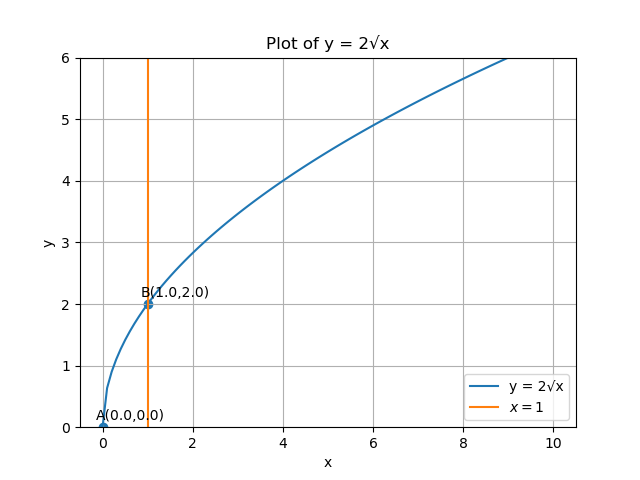
\includegraphics[width=0.5\linewidth]{Fig1.png}
        \caption{Plot of the parabola}
    \end{figure}
    
\end{frame}
\begin{frame}[fragile]
\frametitle{Code(parabola.c)}
\begin{minted}[bgcolor=bg, linenos, fontsize=\small, breaklines]{c}
#include <stdio.h>
#include <math.h>

void compute_values(double* x, double* y, int n) {
    for (int i = 0; i < n; i++) {
        if (x[i] < 0) {
            y[i] = NAN; 
        } else {
            y[i] = 2 * sqrt(x[i]);
        }
    }
}
double compute_value(double x){
	return 2*sqrt(x);
}
\end{minted}
\end{frame}
\begin{frame}[fragile]
  \frametitle{Code(area.c)}

\begin{minted}[bgcolor=bg, linenos, fontsize=\footnotesize, breaklines]{c}
#include <stdio.h>
#include <math.h>
double func(double x){
  return 2*sqrt(x);
}
double computeArea(double a, double b, int n) {
    double delta_x = (b - a) / n; // Step size
    double area = 0.0;
    for (int i = 0; i < n; i++) {
        double x = a + i * delta_x;
        double y = func(x);
        area += y* delta_x; // Add the area of each slice
    }
    return area;
}

\end{minted}
\end{frame}
\begin{frame}[fragile]
  \frametitle{Code(area.c)}

\begin{minted}[bgcolor=bg, linenos, fontsize=\footnotesize, breaklines]{c}
int main(){
  int a=0;
  int b=1;
  FILE *file;
  file =fopen("area.txt","w");
  if (file == NULL) {
        printf("Error opening file!\n");
        return 1; //
    }
  fprintf(file, "The area enclosed by the parabola between the lines x=0 and x=1 is %lf", computeArea(a,b,1000));
  fclose(file);
  return 0;
\end{minted}
\end{frame}
\begin{frame}{Output(area.txt)}
The area enclosed by the parabola between the lines x=0 and x=1 is 1.332320  
\end{frame}
\begin{frame}[fragile]
\frametitle{Code(plot.py)}
\begin{minted}[bgcolor=bg, linenos, fontsize=\scriptsize, breaklines]{python}
import sys                                          
sys.path.insert(0, '/home/john-bobby/MyRepos/matgeo/codes/CoordGeo') 
import numpy as np
import matplotlib.pyplot as plt
import ctypes
from line.funcs import *
from triangle.funcs import *
from conics.funcs import *
math_functions = ctypes.CDLL('./parabola.so')
math_functions.compute_values.argtypes = (ctypes.POINTER(ctypes.c_double), ctypes.POINTER(ctypes.c_double), ctypes.c_int)
math_functions.compute_value.argtypes = [ctypes.c_double]
math_functions.compute_value.restype = ctypes.c_double
x = np.linspace(0, 10, 100)  
y = np.zeros_like(x)
A = np.array(([0, math_functions.compute_value(0)])).reshape(-1, 1)
B = np.array(([1, math_functions.compute_value(1)])).reshape(-1, 1)
C = np.array(([1, -1])).reshape(-1, 1)
D = np.array(([1, 7])).reshape(-1, 1)
x_1 = line_gen(C, D)

\end{minted}
    
\end{frame}
\begin{frame}[fragile]
\frametitle{Code(plot.py)}
\begin{minted}[bgcolor=bg, linenos, fontsize=\scriptsize, breaklines]{python}
math_functions.compute_values(x.ctypes.data_as(ctypes.POINTER(ctypes.c_double))
,y.ctypes.data_as(ctypes.POINTER(ctypes.c_double)), len(x))
points=np.block([[A,B]])
plt.ylim([0, 6]) 
plt.plot(x, y, label='y = 2√x')
plt.plot(x_1[0, :], x_1[1, :], label='$x=1$')
plt.annotate(f"A(0.0,{math_functions.compute_value(0)})", (0, math_functions.compute_value(0)), textcoords="offset points", xytext=(20, 5), ha='center')
plt.annotate(f"B(1.0,{math_functions.compute_value(1)})", (1, math_functions.compute_value(1)), textcoords="offset points", xytext=(20, 5), ha='center')
plt.scatter(tri_coords[0,:], tri_coords[1,:])
plt.title('Plot of y = 2√x')
plt.xlabel('x')
plt.ylabel('y')
plt.legend()
plt.grid()
plt.savefig("/home/john-bobby/MyRepos/EE1030/Assignment5/Figs/Fig1.png")


\end{minted}    
\end{frame}








\end{document}
